

\begin{flushleft}

	\begin{itemize}
		\item byte keyword is an 8-bit signed integer. 
		
		\tabletwo{
			\hline
			Size & \textbf{1 byte (8 bits)} \\
			\hline
			MAX\_VALUE & \textbf{+127} \\
			\hline
			MIN\_VALUE & \textbf{-128} \\
			\hline
			Range & \textbf{-128 to 127} \\
			\hline
		}
		
		\begin{figure}[h!]
			\centering
			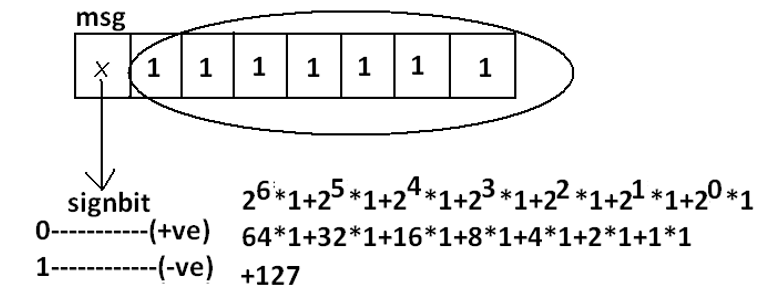
\includegraphics[scale=.4]{content/chapter2/images/byte.png}
		\end{figure}		
		\item Left most bit (also called \textbf{m}ost \textbf{s}ignificant \textbf{b}it) is sign bit , where 
		\begin{itemize}
			\item 0 is positive number
			\item 1 is negative number
		\end{itemize}
		
		\begin{figure}[h!]
			\centering
			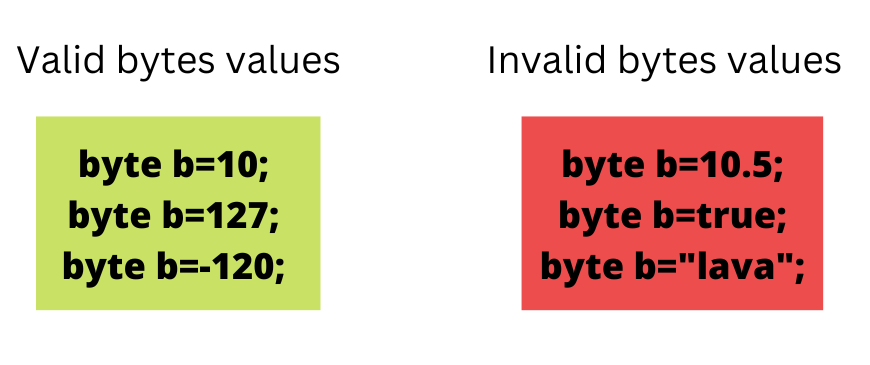
\includegraphics[scale=.45]{content/chapter2/images/byte2.png}
		\end{figure}		
		
	
		\item \textbf{Where is byte used?}
		\begin{itemize}
			\item \textbf{Read/write binary data}
			\item \textbf{Image processing}			
			\item \textbf{Audio processing}
			\item \textbf{Network programming}
		\end{itemize}	
	\end{itemize}
	
\end{flushleft}
